\chapter{Introduction to Attacks On Implementations}
\label{chap:c1_IntroductionAOI}

\section{Motivation} %arbel
\label{sec:Motivation}

The following story is a true story about the NSA – the U.S intelligence agency -  which has an internal and classified, cryptology journal. In the U.S there is a law called “The Freedom of Information Act” (FOIA), which means that, in general, any person can ask access to government documents. So, on 2007, one person went ahead and asked for the table of contents of all the articles in the NSA journal, and the law is the law, so the NSA gave him what he asked, with censorship on some classified titles. After he got that, of course, he asked for the unclassified articles!

The journal, obviously, was used to be secret, but it was approved for release by NSA because of the FOIA law. One article that published in the journal, tells us about something that happened in the years of World War II. In those years, there were some significant developments, and one of them was digital wireless communication. People were able to send themselves messages from one side of the world to the other, using digital signals, but the military forces that used this communication were afraid to be wired by the enemy and to protect those transmissions they had to encrypt them.    

At the end of the encryption process, we get a ciphertext, which can be transmitted without any concern. The obstacle which prevents attackers from decrypting the ciphertext and discover the key is the algorithm which has been written very well.  
Let’s assume we have a weak computer to perform the encryption, because we are in the years of World War II -  no resistors, no iterative circuits – what can the adversary do to find the key?

The adversaries can build a machine which does the decryption – insert the ciphertext into the machine and try all the keys (brute force). But… how do you know which key is the correct one? There is logic to the plaintext – maybe it’s an English, a weather broadcast, an executable – and in general, it’s something you can check the syntax, so with a very high probability, if you get an output that starts with “Heil Hitler” – the key you used to decrypt the ciphertext is the correct key. We need to remember that the encryption machine was not very complex in those years, and to keep the secure massages safe, they had to find a way to protect their ciphertexts. The solution to that issue is a one-time pad.

One-time pad, also called Vernam Cipher, is a simple and powerful encryption system. The idea behind this technique is that the length of the key is the same length as the plain text, and to encrypt you just add them together – if we use digital bits we use XOR, and if we use letters we define an addition operation. It’s called a one-time pad because you can use your pre-shared key only once.

Why does this one-time pad protect from brute force attacks? Because $plaintext \oplus key = ciphertext$ and $ciphertext \oplus key = plaintext$, meaning we can take the ciphertext and any plaintext we want, XOR them together, and get the corresponding random key. In a very secure encryption technique, like AES-256, there are \(2^{256}\) possible keys and with a ciphertext which is 1 MB, we have \(2^{8000000}\) possible keys, but if we don’t know the key there are \(2^{256}\) random plaintext, and maybe just one of them is the real one. The one-time pad has been proven to be completely secure by Claude Shannon, and there is no way to break it.

Back to the years of World War II, to use one-time pad those days, they used machine which called \textbf{AN/FGQ-1 mixer}\cite{cryptoMix} as can be seen in \Cref{fig:Mixer}.

\begin{figure}[htb]
    \centering
    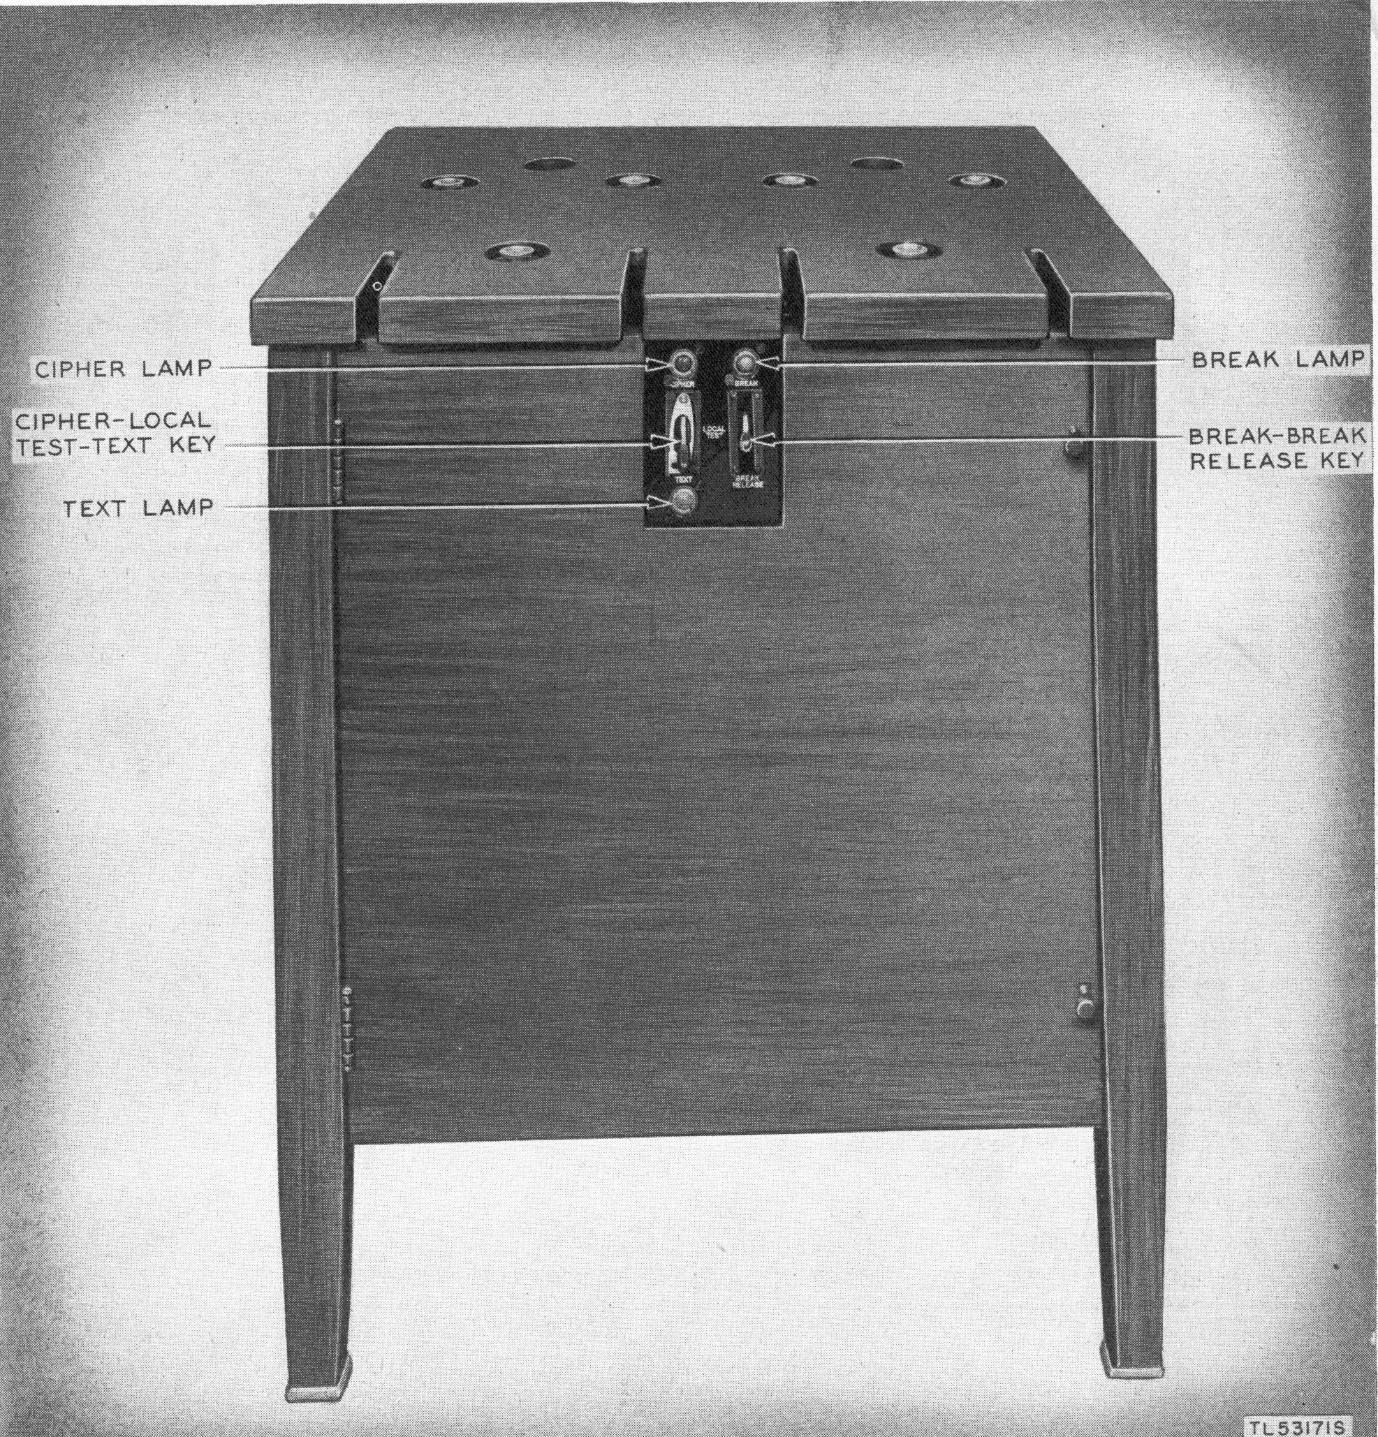
\includegraphics[width=0.8\textwidth]{images/ch1_Intro/MIxer.jpg}
    \caption{\textbf{AN/FGQ-1 Mixer}. Two-way teletypewriter repeater and mixer equipment enclosed in a wooden Table-type cabinet.}
    \label{fig:Mixer}
\end{figure}

This machine is a kind of a box, and next to the box was seat a wireless operator with a typewriter, and the tape that came out from the typewriter was with holes that spooled into the box together with another piece of tape, which was the key. Inside the box were little lights that shine through the holes, and little punches which would punch holes in the third piece of tape – the XOR of the plain text and the key, and this is the output of one operation of the machine. Afterward, the wireless operator feeds the ciphertext into the digital radio to transmit.

Is the machine classified? If the system is designed right - you can reveal the adversary whatever you want except for the secret key, and the system will remain secure.

So, these machines were used during the war, until they break down, and at the time that happened, they have been sent to the Bell Labs (which produced the machines). The engineers who tried to repair one of the machines sat in a room, and on the other side of the room, there was an \textbf{Oscilloscope}. 

An Oscilloscope is like babies monitor - just for signals. You connect the Oscilloscope to an electric circuit, and there is a line that rising every time there is a difference in voltage. \Cref{fig:Oscillo} demonstrates such a setup.
This Oscilloscope was not connected to the mixer, it was just laid at the other side of the room, connected to some other test equipment. The engineers discovered that every time this mixer enter the digit into the tape, they would get a pulse at the Oscilloscope. When you send a current into an electric monitor, the current is moving through the conductor and electromagnetic current is being generated. The Oscilloscope has little wires, and the electromagnetic waves traveling through these wires. As a result, we have a transmit antenna and a receive antenna, so the Oscilloscope measures the holes (the ciphertext) in the tape. Another possible explanation - when the punches punch a hole in the tape, it consumes so much current that the voltage in the room drops a little, and then the lines in the Oscilloscope – without being connected to anything -  just jumps.

\begin{figure}
    \centering
    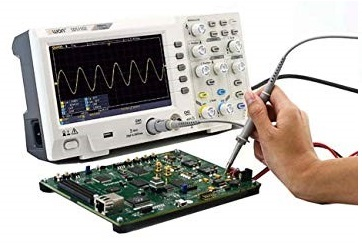
\includegraphics[width=0.8\textwidth]{images/ch1_Intro/oscilloscope.jpg}
    \caption{\textbf{Oscilloscope}. An electronic test instrument which graphically displays varying signal voltages as a function of time.}
    \label{fig:Oscillo}
\end{figure}

The engineers discovered\cite{NSAsecret} that the top-secret information inside this machine was being transmitted over the air. The process the engineers were supposed to do is called responsible disclosure, meaning to report a bug. Like good engineers, they told the Secret Service people about this bug, but they didn't take their diagnosis seriously. So what did they do? The Bell labs were located next to the U.S Secret Service office, so they set up an antenna and they listened for an hour for radio transmissions that the Secret Service got in their office, and they gave the Secret Service their “top-secrets” analyzed massages.
Obviously, the U.S Secret Service realized that the reported attack was not esoteric, and they asked for a solution from the engineers. The solution of Bell labs was to modify the mixers – to surround them in a wire cage which will swallow the radiation that coming out from the machine, to put a shield on the machine (to make sure the power consumption is not affecting the outside), and to make sure that people are not getting close to the machine more than 30 meters. The Secret Service people decided to accept just the distance solution and not the filtering/shielding/isolation solutions, because of the high expenses and time that will cost to modify all the machine during wartime.

In 1954, the Russians published a tender to build military phones. They were very strict about protecting the phones by shielding them and making sure they don’t generate too much radiation. In parallel, they were publishing tenders for things like engines, turbines, etc. and they didn't were so strict for that tenders. This is an evidence to that in those years, the Russians know about the “bug”.
In conclusion, a one-time pad is the most secure cipher known, but from the story above, we can see it was broken. So, what was broken? \textbf{The implementation}.

Here are a couple of other machines which will break using attacks on their implementation:

\begin{itemize}
\item \textbf{Xbox 360}:  Xbox is a PC that plays nothing but games, it is very cheap and you pay for the games. Attackers, obviously, want to crack the Xbox – to play games for free, to watch movies on the device or to run Linux. In Xbox there are some integrity checks, and one of the checks was done by a command called “memory compare”\cite{memcmp}, so you would calculate the integrity check over whatever software it supposes to run and you would have it stored in the secure memory, and then you would try to compare using these 2 values. This command leaks the length of the number of correct bytes before the first incorrect byte, so if you compare 2 blocks and the first bit is different – the response will be fast, and if the blocks identical until the very last bit – it would take a longer. This is one of the things that was enough to break the machine. 
\item \textbf{Oyster Card}: it’s a computer without power supply and Inside this computer that are stored values. Attackers could attack this card to take the train for free. There are a lot of ways to attack the implantation of that card. \cite{garcia2008dismantling, courtois2008algebraic}
\item \textbf{Car Keys}\cite{relayAttack}
\item \textbf{FPGA}\cite{fpga}: a piece of hardware which is a very versatile, meaning we can find it many kinds of hardware – routers, audio equipment, spaceships, etc. the FPGA has a firmware installed inside, and if you want to copy some designs you need to find the firmware. The firmware is encrypted, but a bunch of Germans researches discovered\cite{moradi2011vulnerability} that if you measure the power consumption of the FPGA while it is encrypting the firmware – you can find out what is the key.
\end{itemize}

When we implement an algorithm without being careful, we can be exposed to implementation attacks. To protects against these attacks, we must protect the implementation and do countermeasures, but as we saw at World War II, those countermeasures have a price, thus making the system more expensive, and they make the system heavier.

\section{System Implementation}
\label{sec:SystemImpl}

The simplest form of a computational system is a device which gets input, makes a computation and finally produces an output as can be seen in \Cref{fig:SecDev1}. We assume that our system contains a secret, which cannot be revealed to anyone before, during and after the computation process. 

\begin{figure}[htb]
    \centering
    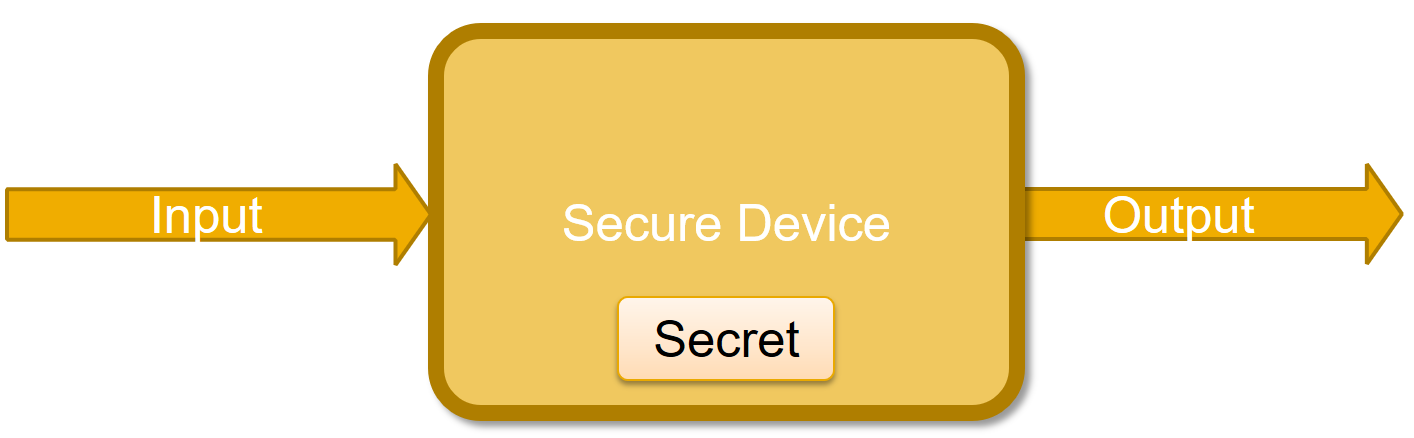
\includegraphics[width=0.8\textwidth]{images/ch1_Intro/Secure_device1.png}
    \caption{\textbf{Simplest Model}. The device make a computation using the secret and the input, and outputs the result.}
    \label{fig:SecDev1}
\end{figure}

But, if that all what the “system” has, it is not a system, it is just an Algorithm. What turns an algorithm to be a system? It’s implementation.

Think about ATM – very simple device without cryptography. The input is our credit card and a 4-digits PIN code, the output is money. If we don’t know the PIN code we can go over the all possible combinations of 4-digits code (brute force), and finally find the correct PIN. Unfortunately, we have a limit of 3 trials until the card is being shredded. What an attacker can do?

As an output, and besides the money, we have also some additional outputs which have been produced by the implementation of the physical system. Those additional outputs are called "Side Channels" and they are outputs which the system designer did not intend to produce. Those outputs are demonstrated in \Cref{fig:SecDev2}

\begin{figure}[htb]
    \centering
    \cent
    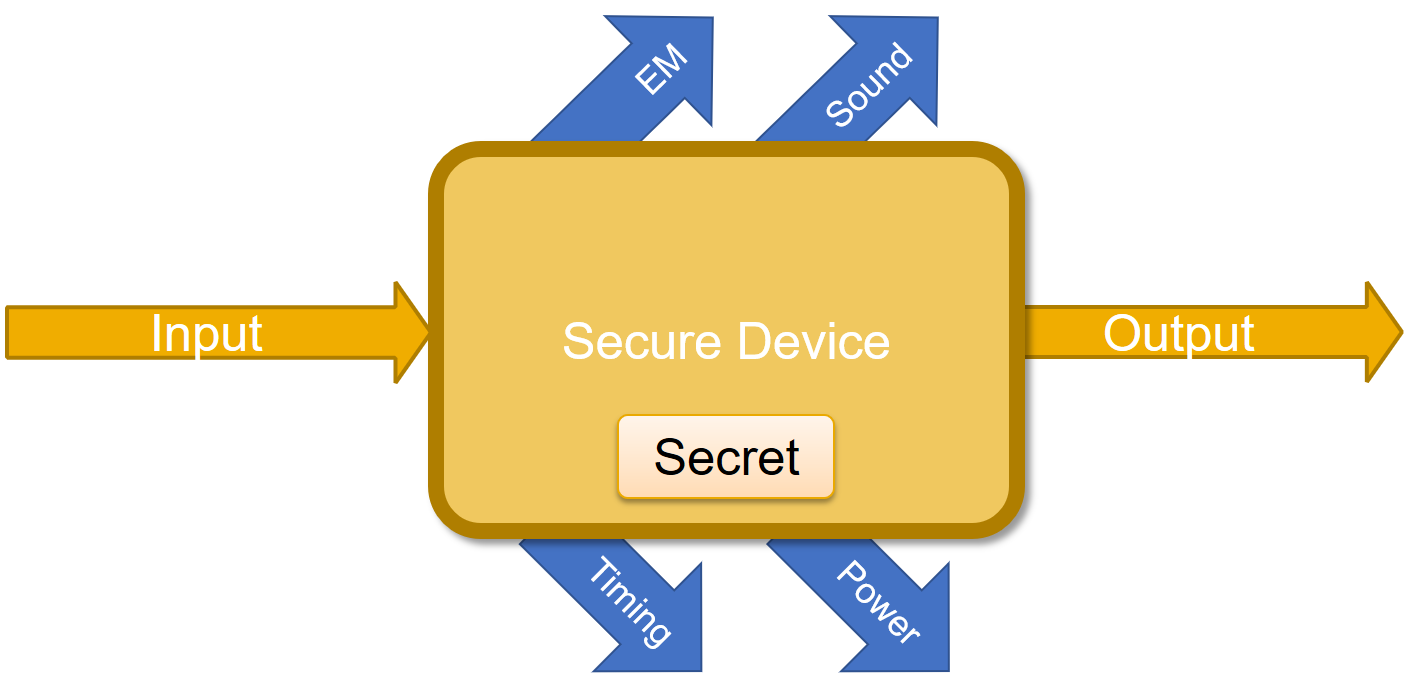
\includegraphics[width=0.8\textwidth]{images/ch1_Intro/Secure_device2.png}
    \caption{\textbf{Side Channels of the System}. Caused by the implementation of the system}
    \label{fig:SecDev2}
\end{figure}

For example, we can measure the time it takes to fulfill the operation, electromagnetic radiation, the sound of the device while the operation is being fulfilled, power measurements, etc. These are \textbf{Passive Attacks} – meaning we are letting the device to do his stuff while we just listening.

There are also \textbf{Active Attacks} – called also fault attacks -  try to break the device in a way that it will be "just a little broken" – ruin the device's activity in some way. It can be by turn it off in the middle of calculation, change his clock, etc. As a result, we will maybe not get the actual secret, but we will get some kind of errors that can teach us a lot about the secret. 

\begin{figure}[htb]
    \centering
    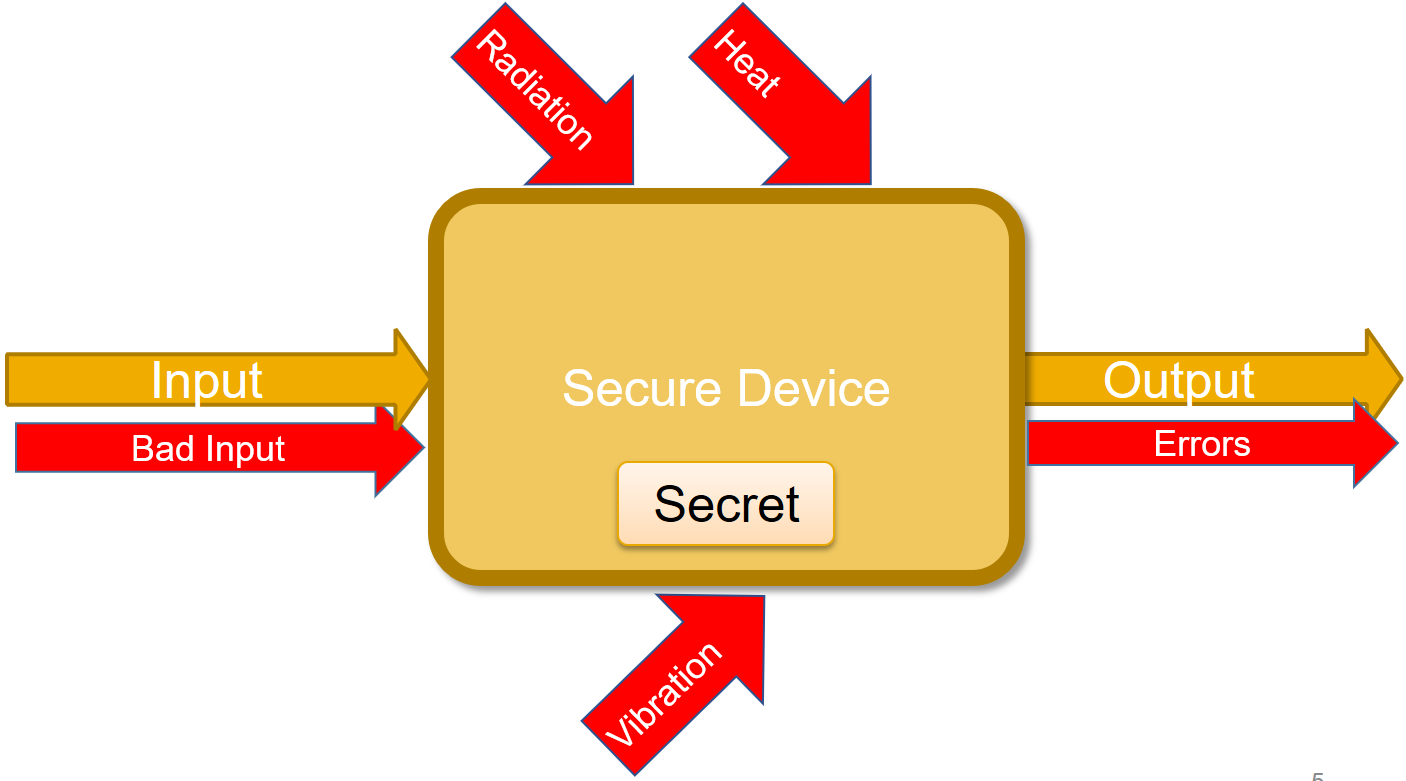
\includegraphics[width=0.8\textwidth]{images/ch1_Intro/Secure_device3.png}
    \caption{\textbf{Fault Attacks}. Manipulating the device through side channels}
    \label{fig:SecDev3}
\end{figure}

\section{Security of a System}
\label{sec:SystemSecurity}

When we can say that a system is secured?
Usually, we define a system as a "secured system" if the system maintains three aspects of information security, known as the CIA\cite{cia} triad:

\begin{itemize}
\item \textbf{Confidentiality} - when you are interacting with a system, you only get what you wanted to get. For instance, when I check my test grade, I’ll get my grade and not my friend’s grade. A possible attack could be data leakage.
\item \textbf{Integrity} - all the data in the system is correct. A possible attack could be that one side of the communication will accept a massage they are not supposed to accept.
\item \textbf{Availability} - the system must work (in a reasonable time). A possible attack could be a Denial of Service (DOS).
\end{itemize}

In \Cref{fig:CIA} the relation between those aspects is demonstrated as the Triangle of Information Security.

We don’t have to use cryptography to secure our system. For example, if someone goes to some event without invitation, there is a security to prevent him from getting in.

An \textbf{Algorithm} is a process or set of rules to be followed in calculations or other problem-solving operations. An example of an algorithm is GCD/Extended GCD. An algorithm is secure when it is implementing the CIA triad mentioned above.    
A \textbf{Protocol} is when you need to get something done, for example, AES -  the input is a 128-bit key and a 16-bytes plaintext (in case of more than 16-bytes we should use padding), and the output is a ciphertext.

\begin{figure}
    \centering
    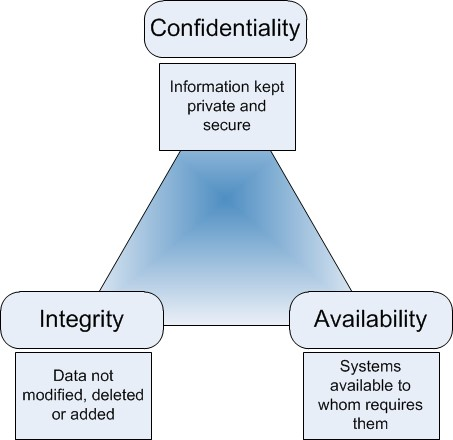
\includegraphics[width=0.5\textwidth]{images/ch1_Intro/cia.jpg}
    \caption{\textbf{CIA Triangle}. The classic model for information security. Defines three objectives of security: maintaining confidentiality, integrity, and availability. Each objective addresses a different aspect of providing protection for information.}
    \label{fig:CIA}
\end{figure}

The millionaire problem\cite{lin2005efficient} is a classic problem by Yao and it is an example of a protocol – this problem asks whether two millionaires can learn who is richer, without revealing to one another how much money they each have. One possible solution, they could invite a poor man, tell him in secret how much money each has, and the poor man will announce who is richer.  

Cryptographically Secure Algorithms and Protocols:
\begin{itemize}
\item \textbf{Encryption and Decryption} - Public key-RSA, Symmetric key-AES
\item \textbf{Signing and verification} - must be an asymmetric key. There are 2 parties – signing party and verifying party (who gets the public key). The difference between signing and decryption is when one side sends a signed message it comes with a signature, and when one side decrypts a message he is sending only the ciphertext.
\item \textbf{Key Exchange} - Diffie Hellman algorithm.
\item \textbf{Hashing and HMACs} - a hash is a function that gets a long input (the length doesn’t matter) and outputs a fixed size output. A hash function is secure when it’s hard to find collisions, e.g. 2 massages with the same hash. HMAC is a hash with a key – when you change the key, the hash is changed.
\item \textbf{Multiparty Computation}
\item \textbf{Cryptocurrency}
\end{itemize}

Secure Architectures without cryptography:
\begin{itemize}
\item \textbf{Secure Policies} - like access control to a military base, for instance.
\item \textbf{User Separation and Sandboxing} -a program is divided into parts which are limited to the specific privileges they require to perform a specific task.
\item \textbf{Virtual Memory} - application has a view of the memory, and we can take to pointer and point to some parts of the memory. We will get our old memory (which I’m allowed) or the app will crash due to access to invalid memory space. In theory, we can’t get another user memory.
\end{itemize}

\section{Constructing and Using a Threat Model}
\label{sec:BreakImpl}

What is the main advantage we have as attackers which allowed us to break implementations that are secure in theory?
The main advantage is that we have more inputs and outputs – side channels, leakage – and together it means that we can break a completely secure algorithm. 
But when is an algorithm’s implementation secure? CIA triad still holds, but the thing that missing here is the \textbf{story}, i.e. what are we allowing the adversary to do with my system – the more power we give the adversary the attack becomes less impressive. 

Let’s have a look at a little system where the assumptions were broken:

\begin{figure}[htb]
    \centering
    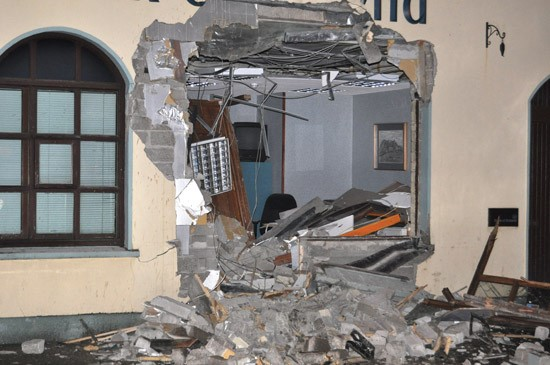
\includegraphics[width=0.8\textwidth]{images/ch1_Intro/Bank.jpg}
    \caption{\textbf{ATM theft.} The thieves simply ripped the machine out of the wall.}
    \label{fig:Bank}
\end{figure}

\Cref{fig:Bank} presents a wall of a bank in Ireland, which an ATM was constructed on it. As we know, the ATMs are very secure systems – they have encryption, they check our ID very carefully and if we make any mistake they shred the card. What happened is that the ATM was stolen from the wall of a bank by thieves which took a digger and smashed through the wall, put the ATM on their track, and laid the digger across the road to prevent the police from chasing them. We can learn from this story, that the ATM was secure, but their threat model was wrong.

The most important thing about the threat model is the story. If the story is a thief which comes to the bank in the middle of the night with a digger it’s one story, and if a thief comes in the middle of the day by foot, it’s a different story. Once we have the story, we can detail what are the properties of the story. We divide them as follows:

\begin{itemize}
    \item \textbf{Victim Assets} - what the victim have that I want to steel? 
        \begin{itemize}
            \item \textbf{Cryptographic secretes (keys)} -  the keys are short, and when one steals the key – the attack has succeeded. There are two kinds of keys, long term, and short term.
                \begin{itemize}
                    \item \textbf{Long term key } - the private key that identifies a server. If one steals this key, he will be able to sign malware as a software update.
                    \item \textbf{Short term key} - a key that generated during a session start from the long-term key. If one steals this key, he can decode all the massages in the current session and modify/inject them.
                \end{itemize}
                Notice that if one steals the long-term key it doesn’t mean he can steal the short-term key.
            \item \textbf{State secrets} - for example, ASLR or configuration of a system. If one can find out the addresses of functions in the memory of a victim, he can write exploits. 
            \item \textbf{Human secrets} - things which the users do not want to expose like passwords, medical condition, etc.
        \end{itemize}
    \item \textbf{Attacker Capabilities} - what can the attacker do?
        \begin{itemize}
            \item \textbf{Off-path} - the attacker sitting somewhere in the world – can’t observe or communicate with you, but he can attack you somehow. 
            \item \textbf{Passive Man in the Middle} - attacker who can see the victim communication with the server, for example, but he cannot communicate with the victim directly.
            \item \textbf{Active Man in the Middle} - an attacker who can interact with the server and can do replay attacks.
            \item \textbf{Physical Access} - an attacker who has physical access to the victim. For example, removing or unplugging or melting stuff in the system.
        \end{itemize}
        An important thing we need to consider when we are talking about attacker capabilities is the other defenses we must protect our system – guard or camera, for example.
        Another thing is the scale of the attack – how many systems can we attack at once. If the attack is physical, probably just one system. If the attacker attacks from an android app, maybe he can attack all the phones in the world.
    \item \textbf{Attacker Objectives} - who are the attackers? What do they want?
        \begin{itemize}
            \item \textbf{Stealing stuff} - the attacker might want to steal your secrets.
            \item \textbf{Duplicating stuff} - for example, the attacker can buy one smart TV card, and generate a thousand duplicates from this card to sell them. 
            \item \textbf{Forging stuff} - the attacker creates something new, driver licenses for instance.
            \item \textbf{Corrupting stuff} - the attacker breaks something and decommissioned the system.
        \end{itemize}
\end{itemize}

Of course, the more limits we put on the attacker, the attack gets more and more impressive.
